\DeclareFixedFont{\titlefont}{T1}{ppl}{b}{}{0.5in}
\DeclareFixedFont{\subtitlefont}{T1}{ppl}{b}{}{0.3in}
\DeclareFixedFont{\versionfont}{T1}{ppl}{}{}{0.2in}
\newgeometry{left=1in, right=1in,top=1in, bottom=0in}
\definecolor{mytan}{HTML}{F6D5A8}
\pagecolor{mytan}

\thispagestyle{empty}
\begin{flushright}
  \titlefont Informatics for\\[9pt] complete beginners\\[12pt]
  \subtitlefont Gavin Sinclair
  \vfill
  \versionfont \BookVersionString \\[6pt] \BookVersionDate
  \vfill
\end{flushright}

\begin{center}
  \begin{tikzpicture}
    \node[scope fading=north, inner sep=0pt, outer sep=0pt]{
       \makebox[\textwidth]{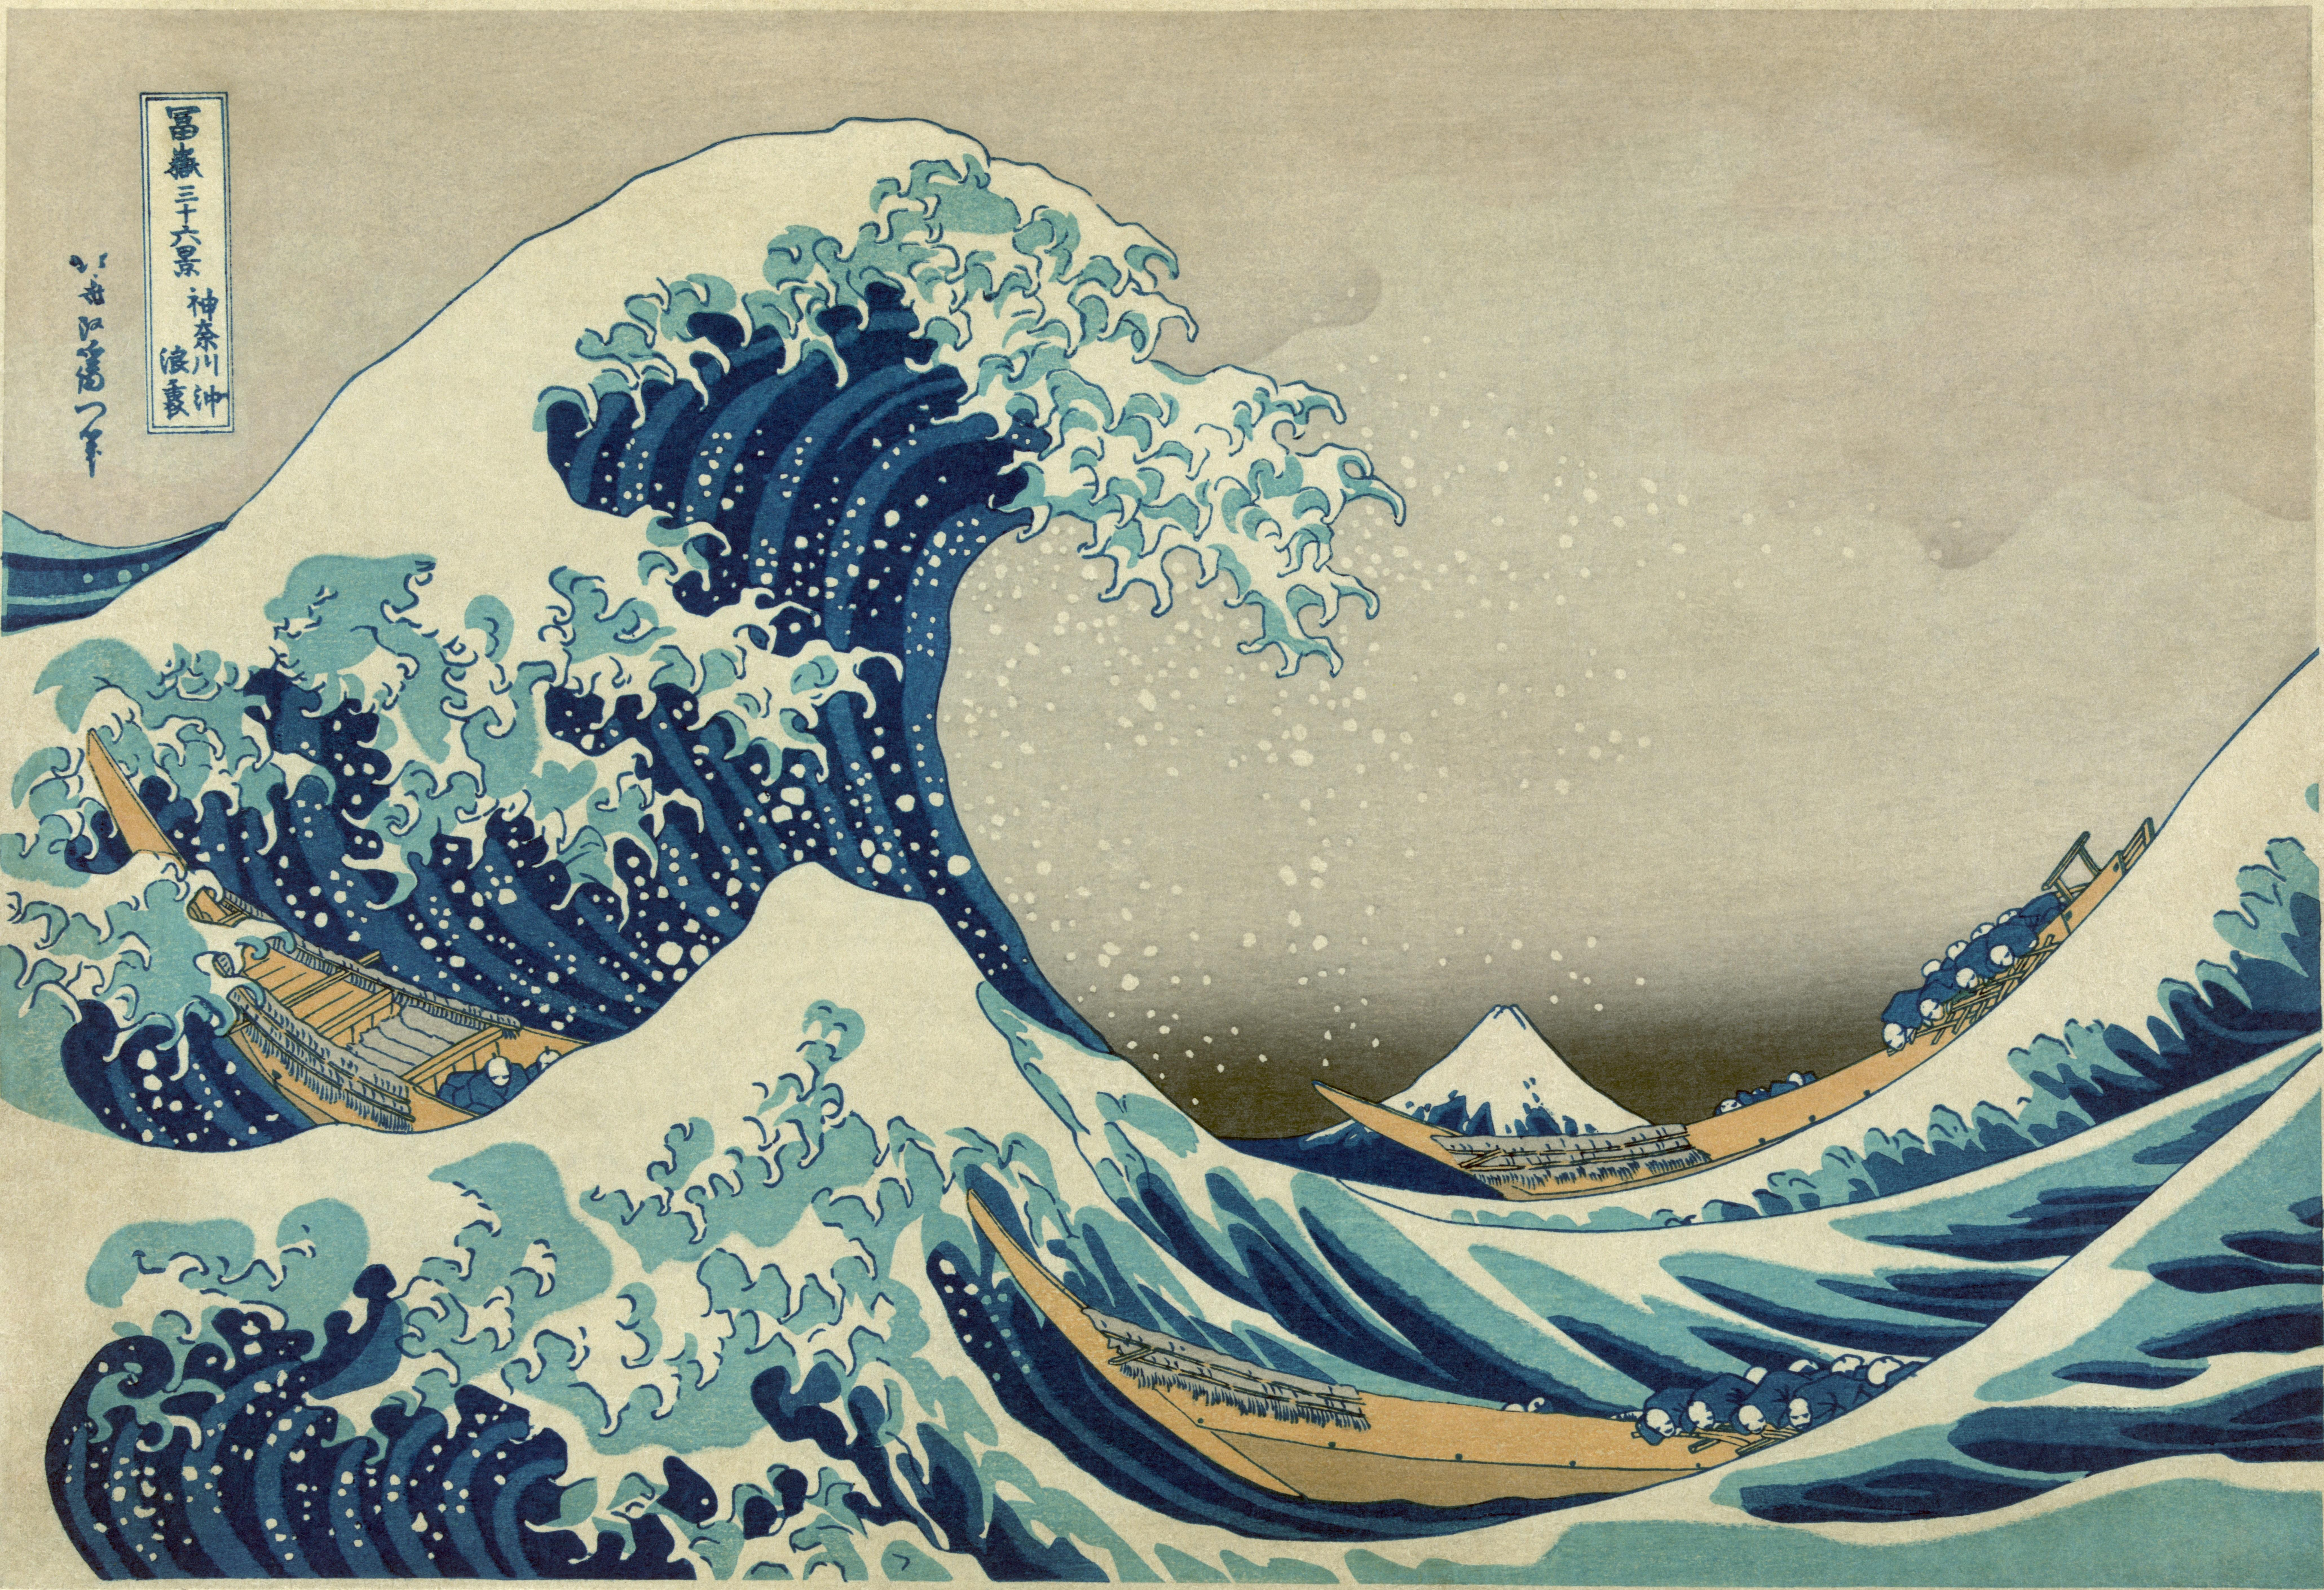
\includegraphics[width=\paperwidth]{images/kanagawa-wave.jpg}}
     };
   \end{tikzpicture}
 \end{center}
